% Created by tikzDevice version 0.12.3 on 2020-04-21 11:12:06
% !TEX encoding = UTF-8 Unicode
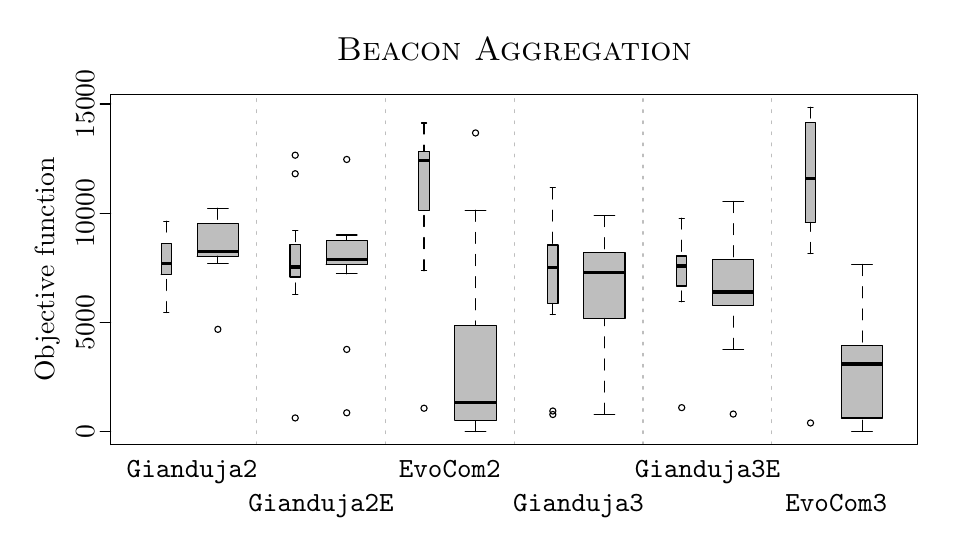
\begin{tikzpicture}[x=1pt,y=1pt]
\definecolor{fillColor}{RGB}{255,255,255}
\path[use as bounding box,fill=fillColor,fill opacity=0.00] (0,0) rectangle (325.21,180.67);
\begin{scope}
\path[clip] ( 30.00, 30.00) rectangle (321.61,156.67);
\definecolor{fillColor}{RGB}{190,190,190}

\path[fill=fillColor] ( 48.25, 91.49) --
	( 51.97, 91.49) --
	( 51.97,102.81) --
	( 48.25,102.81) --
	cycle;
\definecolor{drawColor}{RGB}{0,0,0}

\path[draw=drawColor,line width= 1.2pt,line join=round] ( 48.25, 95.37) -- ( 51.97, 95.37);

\path[draw=drawColor,line width= 0.4pt,dash pattern=on 4pt off 4pt ,line join=round,line cap=round] ( 50.11, 77.71) -- ( 50.11, 91.49);

\path[draw=drawColor,line width= 0.4pt,dash pattern=on 4pt off 4pt ,line join=round,line cap=round] ( 50.11,110.77) -- ( 50.11,102.81);

\path[draw=drawColor,line width= 0.4pt,line join=round,line cap=round] ( 49.18, 77.71) -- ( 51.04, 77.71);

\path[draw=drawColor,line width= 0.4pt,line join=round,line cap=round] ( 49.18,110.77) -- ( 51.04,110.77);

\path[draw=drawColor,line width= 0.4pt,line join=round,line cap=round] ( 48.25, 91.49) --
	( 51.97, 91.49) --
	( 51.97,102.81) --
	( 48.25,102.81) --
	( 48.25, 91.49);

\path[fill=fillColor] ( 61.28, 98.12) --
	( 76.18, 98.12) --
	( 76.18,109.85) --
	( 61.28,109.85) --
	cycle;

\path[draw=drawColor,line width= 1.2pt,line join=round] ( 61.28, 99.86) -- ( 76.18, 99.86);

\path[draw=drawColor,line width= 0.4pt,dash pattern=on 4pt off 4pt ,line join=round,line cap=round] ( 68.73, 95.49) -- ( 68.73, 98.12);

\path[draw=drawColor,line width= 0.4pt,dash pattern=on 4pt off 4pt ,line join=round,line cap=round] ( 68.73,115.42) -- ( 68.73,109.85);

\path[draw=drawColor,line width= 0.4pt,line join=round,line cap=round] ( 65.01, 95.49) -- ( 72.46, 95.49);

\path[draw=drawColor,line width= 0.4pt,line join=round,line cap=round] ( 65.01,115.42) -- ( 72.46,115.42);

\path[draw=drawColor,line width= 0.4pt,line join=round,line cap=round] ( 61.28, 98.12) --
	( 76.18, 98.12) --
	( 76.18,109.85) --
	( 61.28,109.85) --
	( 61.28, 98.12);

\path[draw=drawColor,line width= 0.4pt,line join=round,line cap=round] ( 68.73, 71.66) circle (  1.12);

\path[fill=fillColor] ( 94.80, 90.59) --
	( 98.53, 90.59) --
	( 98.53,102.16) --
	( 94.80,102.16) --
	cycle;

\path[draw=drawColor,line width= 1.2pt,line join=round] ( 94.80, 94.22) -- ( 98.53, 94.22);

\path[draw=drawColor,line width= 0.4pt,dash pattern=on 4pt off 4pt ,line join=round,line cap=round] ( 96.67, 84.40) -- ( 96.67, 90.59);

\path[draw=drawColor,line width= 0.4pt,dash pattern=on 4pt off 4pt ,line join=round,line cap=round] ( 96.67,107.33) -- ( 96.67,102.16);

\path[draw=drawColor,line width= 0.4pt,line join=round,line cap=round] ( 95.73, 84.40) -- ( 97.60, 84.40);

\path[draw=drawColor,line width= 0.4pt,line join=round,line cap=round] ( 95.73,107.33) -- ( 97.60,107.33);

\path[draw=drawColor,line width= 0.4pt,line join=round,line cap=round] ( 94.80, 90.59) --
	( 98.53, 90.59) --
	( 98.53,102.16) --
	( 94.80,102.16) --
	( 94.80, 90.59);

\path[draw=drawColor,line width= 0.4pt,line join=round,line cap=round] ( 96.67, 39.65) circle (  1.12);

\path[draw=drawColor,line width= 0.4pt,line join=round,line cap=round] ( 96.67,127.88) circle (  1.12);

\path[draw=drawColor,line width= 0.4pt,line join=round,line cap=round] ( 96.67,134.59) circle (  1.12);

\path[fill=fillColor] (107.84, 95.06) --
	(122.74, 95.06) --
	(122.74,103.85) --
	(107.84,103.85) --
	cycle;

\path[draw=drawColor,line width= 1.2pt,line join=round] (107.84, 96.95) -- (122.74, 96.95);

\path[draw=drawColor,line width= 0.4pt,dash pattern=on 4pt off 4pt ,line join=round,line cap=round] (115.29, 91.72) -- (115.29, 95.06);

\path[draw=drawColor,line width= 0.4pt,dash pattern=on 4pt off 4pt ,line join=round,line cap=round] (115.29,105.74) -- (115.29,103.85);

\path[draw=drawColor,line width= 0.4pt,line join=round,line cap=round] (111.56, 91.72) -- (119.01, 91.72);

\path[draw=drawColor,line width= 0.4pt,line join=round,line cap=round] (111.56,105.74) -- (119.01,105.74);

\path[draw=drawColor,line width= 0.4pt,line join=round,line cap=round] (107.84, 95.06) --
	(122.74, 95.06) --
	(122.74,103.85) --
	(107.84,103.85) --
	(107.84, 95.06);

\path[draw=drawColor,line width= 0.4pt,line join=round,line cap=round] (115.29, 41.50) circle (  1.12);

\path[draw=drawColor,line width= 0.4pt,line join=round,line cap=round] (115.29,133.05) circle (  1.12);

\path[draw=drawColor,line width= 0.4pt,line join=round,line cap=round] (115.29, 64.41) circle (  1.12);

\path[fill=fillColor] (141.36,114.71) --
	(145.08,114.71) --
	(145.08,135.99) --
	(141.36,135.99) --
	cycle;

\path[draw=drawColor,line width= 1.2pt,line join=round] (141.36,132.57) -- (145.08,132.57);

\path[draw=drawColor,line width= 0.4pt,dash pattern=on 4pt off 4pt ,line join=round,line cap=round] (143.22, 92.83) -- (143.22,114.71);

\path[draw=drawColor,line width= 0.4pt,dash pattern=on 4pt off 4pt ,line join=round,line cap=round] (143.22,146.23) -- (143.22,135.99);

\path[draw=drawColor,line width= 0.4pt,line join=round,line cap=round] (142.29, 92.83) -- (144.15, 92.83);

\path[draw=drawColor,line width= 0.4pt,line join=round,line cap=round] (142.29,146.23) -- (144.15,146.23);

\path[draw=drawColor,line width= 0.4pt,line join=round,line cap=round] (141.36,114.71) --
	(145.08,114.71) --
	(145.08,135.99) --
	(141.36,135.99) --
	(141.36,114.71);

\path[draw=drawColor,line width= 0.4pt,line join=round,line cap=round] (143.22, 43.15) circle (  1.12);

\path[fill=fillColor] (154.39, 38.87) --
	(169.29, 38.87) --
	(169.29, 73.12) --
	(154.39, 73.12) --
	cycle;

\path[draw=drawColor,line width= 1.2pt,line join=round] (154.39, 45.26) -- (169.29, 45.26);

\path[draw=drawColor,line width= 0.4pt,dash pattern=on 4pt off 4pt ,line join=round,line cap=round] (161.84, 34.69) -- (161.84, 38.87);

\path[draw=drawColor,line width= 0.4pt,dash pattern=on 4pt off 4pt ,line join=round,line cap=round] (161.84,114.71) -- (161.84, 73.12);

\path[draw=drawColor,line width= 0.4pt,line join=round,line cap=round] (158.12, 34.69) -- (165.57, 34.69);

\path[draw=drawColor,line width= 0.4pt,line join=round,line cap=round] (158.12,114.71) -- (165.57,114.71);

\path[draw=drawColor,line width= 0.4pt,line join=round,line cap=round] (154.39, 38.87) --
	(169.29, 38.87) --
	(169.29, 73.12) --
	(154.39, 73.12) --
	(154.39, 38.87);

\path[draw=drawColor,line width= 0.4pt,line join=round,line cap=round] (161.84,142.63) circle (  1.12);

\path[fill=fillColor] (187.91, 81.06) --
	(191.64, 81.06) --
	(191.64,102.13) --
	(187.91,102.13) --
	cycle;

\path[draw=drawColor,line width= 1.2pt,line join=round] (187.91, 93.92) -- (191.64, 93.92);

\path[draw=drawColor,line width= 0.4pt,dash pattern=on 4pt off 4pt ,line join=round,line cap=round] (189.77, 77.00) -- (189.77, 81.06);

\path[draw=drawColor,line width= 0.4pt,dash pattern=on 4pt off 4pt ,line join=round,line cap=round] (189.77,122.76) -- (189.77,102.13);

\path[draw=drawColor,line width= 0.4pt,line join=round,line cap=round] (188.84, 77.00) -- (190.70, 77.00);

\path[draw=drawColor,line width= 0.4pt,line join=round,line cap=round] (188.84,122.76) -- (190.70,122.76);

\path[draw=drawColor,line width= 0.4pt,line join=round,line cap=round] (187.91, 81.06) --
	(191.64, 81.06) --
	(191.64,102.13) --
	(187.91,102.13) --
	(187.91, 81.06);

\path[draw=drawColor,line width= 0.4pt,line join=round,line cap=round] (189.77, 40.89) circle (  1.12);

\path[draw=drawColor,line width= 0.4pt,line join=round,line cap=round] (189.77, 42.15) circle (  1.12);

\path[fill=fillColor] (200.95, 75.59) --
	(215.84, 75.59) --
	(215.84, 99.28) --
	(200.95, 99.28) --
	cycle;

\path[draw=drawColor,line width= 1.2pt,line join=round] (200.95, 92.22) -- (215.84, 92.22);

\path[draw=drawColor,line width= 0.4pt,dash pattern=on 4pt off 4pt ,line join=round,line cap=round] (208.40, 40.97) -- (208.40, 75.59);

\path[draw=drawColor,line width= 0.4pt,dash pattern=on 4pt off 4pt ,line join=round,line cap=round] (208.40,112.77) -- (208.40, 99.28);

\path[draw=drawColor,line width= 0.4pt,line join=round,line cap=round] (204.67, 40.97) -- (212.12, 40.97);

\path[draw=drawColor,line width= 0.4pt,line join=round,line cap=round] (204.67,112.77) -- (212.12,112.77);

\path[draw=drawColor,line width= 0.4pt,line join=round,line cap=round] (200.95, 75.59) --
	(215.84, 75.59) --
	(215.84, 99.28) --
	(200.95, 99.28) --
	(200.95, 75.59);

\path[fill=fillColor] (234.47, 87.34) --
	(238.19, 87.34) --
	(238.19, 98.15) --
	(234.47, 98.15) --
	cycle;

\path[draw=drawColor,line width= 1.2pt,line join=round] (234.47, 94.58) -- (238.19, 94.58);

\path[draw=drawColor,line width= 0.4pt,dash pattern=on 4pt off 4pt ,line join=round,line cap=round] (236.33, 81.57) -- (236.33, 87.34);

\path[draw=drawColor,line width= 0.4pt,dash pattern=on 4pt off 4pt ,line join=round,line cap=round] (236.33,111.85) -- (236.33, 98.15);

\path[draw=drawColor,line width= 0.4pt,line join=round,line cap=round] (235.40, 81.57) -- (237.26, 81.57);

\path[draw=drawColor,line width= 0.4pt,line join=round,line cap=round] (235.40,111.85) -- (237.26,111.85);

\path[draw=drawColor,line width= 0.4pt,line join=round,line cap=round] (234.47, 87.34) --
	(238.19, 87.34) --
	(238.19, 98.15) --
	(234.47, 98.15) --
	(234.47, 87.34);

\path[draw=drawColor,line width= 0.4pt,line join=round,line cap=round] (236.33, 43.37) circle (  1.12);

\path[fill=fillColor] (247.50, 80.36) --
	(262.40, 80.36) --
	(262.40, 96.92) --
	(247.50, 96.92) --
	cycle;

\path[draw=drawColor,line width= 1.2pt,line join=round] (247.50, 85.16) -- (262.40, 85.16);

\path[draw=drawColor,line width= 0.4pt,dash pattern=on 4pt off 4pt ,line join=round,line cap=round] (254.95, 64.43) -- (254.95, 80.36);

\path[draw=drawColor,line width= 0.4pt,dash pattern=on 4pt off 4pt ,line join=round,line cap=round] (254.95,117.88) -- (254.95, 96.92);

\path[draw=drawColor,line width= 0.4pt,line join=round,line cap=round] (251.23, 64.43) -- (258.67, 64.43);

\path[draw=drawColor,line width= 0.4pt,line join=round,line cap=round] (251.23,117.88) -- (258.67,117.88);

\path[draw=drawColor,line width= 0.4pt,line join=round,line cap=round] (247.50, 80.36) --
	(262.40, 80.36) --
	(262.40, 96.92) --
	(247.50, 96.92) --
	(247.50, 80.36);

\path[draw=drawColor,line width= 0.4pt,line join=round,line cap=round] (254.95, 41.05) circle (  1.12);

\path[fill=fillColor] (281.02,110.29) --
	(284.74,110.29) --
	(284.74,146.35) --
	(281.02,146.35) --
	cycle;

\path[draw=drawColor,line width= 1.2pt,line join=round] (281.02,126.06) -- (284.74,126.06);

\path[draw=drawColor,line width= 0.4pt,dash pattern=on 4pt off 4pt ,line join=round,line cap=round] (282.88, 99.06) -- (282.88,110.29);

\path[draw=drawColor,line width= 0.4pt,dash pattern=on 4pt off 4pt ,line join=round,line cap=round] (282.88,151.98) -- (282.88,146.35);

\path[draw=drawColor,line width= 0.4pt,line join=round,line cap=round] (281.95, 99.06) -- (283.81, 99.06);

\path[draw=drawColor,line width= 0.4pt,line join=round,line cap=round] (281.95,151.98) -- (283.81,151.98);

\path[draw=drawColor,line width= 0.4pt,line join=round,line cap=round] (281.02,110.29) --
	(284.74,110.29) --
	(284.74,146.35) --
	(281.02,146.35) --
	(281.02,110.29);

\path[draw=drawColor,line width= 0.4pt,line join=round,line cap=round] (282.88, 37.83) circle (  1.12);

\path[fill=fillColor] (294.05, 39.62) --
	(308.95, 39.62) --
	(308.95, 65.75) --
	(294.05, 65.75) --
	cycle;

\path[draw=drawColor,line width= 1.2pt,line join=round] (294.05, 59.14) -- (308.95, 59.14);

\path[draw=drawColor,line width= 0.4pt,dash pattern=on 4pt off 4pt ,line join=round,line cap=round] (301.50, 34.81) -- (301.50, 39.62);

\path[draw=drawColor,line width= 0.4pt,dash pattern=on 4pt off 4pt ,line join=round,line cap=round] (301.50, 95.08) -- (301.50, 65.75);

\path[draw=drawColor,line width= 0.4pt,line join=round,line cap=round] (297.78, 34.81) -- (305.23, 34.81);

\path[draw=drawColor,line width= 0.4pt,line join=round,line cap=round] (297.78, 95.08) -- (305.23, 95.08);

\path[draw=drawColor,line width= 0.4pt,line join=round,line cap=round] (294.05, 39.62) --
	(308.95, 39.62) --
	(308.95, 65.75) --
	(294.05, 65.75) --
	(294.05, 39.62);
\definecolor{drawColor}{RGB}{190,190,190}

\path[draw=drawColor,line width= 0.4pt,dash pattern=on 1pt off 3pt ,line join=round,line cap=round] ( 82.70, 30.00) -- ( 82.70,156.67);

\path[draw=drawColor,line width= 0.4pt,dash pattern=on 1pt off 3pt ,line join=round,line cap=round] (129.25, 30.00) -- (129.25,156.67);

\path[draw=drawColor,line width= 0.4pt,dash pattern=on 1pt off 3pt ,line join=round,line cap=round] (175.81, 30.00) -- (175.81,156.67);

\path[draw=drawColor,line width= 0.4pt,dash pattern=on 1pt off 3pt ,line join=round,line cap=round] (222.36, 30.00) -- (222.36,156.67);

\path[draw=drawColor,line width= 0.4pt,dash pattern=on 1pt off 3pt ,line join=round,line cap=round] (268.92, 30.00) -- (268.92,156.67);
\end{scope}
\begin{scope}
\path[clip] (  0.00,  0.00) rectangle (325.21,180.67);
\definecolor{drawColor}{RGB}{0,0,0}

\node[text=drawColor,anchor=base,inner sep=0pt, outer sep=0pt, scale=  1.00] at ( 59.42, 18.00) {\texttt{Gianduja2}};

\node[text=drawColor,anchor=base,inner sep=0pt, outer sep=0pt, scale=  1.00] at (152.53, 18.00) {\texttt{EvoCom2}};

\node[text=drawColor,anchor=base,inner sep=0pt, outer sep=0pt, scale=  1.00] at (245.64, 18.00) {\texttt{Gianduja3E}};

\node[text=drawColor,anchor=base,inner sep=0pt, outer sep=0pt, scale=  1.00] at (105.98,  6.00) {\texttt{Gianduja2E}};

\node[text=drawColor,anchor=base,inner sep=0pt, outer sep=0pt, scale=  1.00] at (199.08,  6.00) {\texttt{Gianduja3}};

\node[text=drawColor,anchor=base,inner sep=0pt, outer sep=0pt, scale=  1.00] at (292.19,  6.00) {\texttt{EvoCom3}};
\end{scope}
\begin{scope}
\path[clip] (  0.00,  0.00) rectangle (325.21,180.67);
\definecolor{drawColor}{RGB}{0,0,0}

\node[text=drawColor,anchor=base,inner sep=0pt, outer sep=0pt, scale=  1.20] at (175.81,168.67) {\textsc{Beacon Aggregation}};

\node[text=drawColor,rotate= 90.00,anchor=base,inner sep=0pt, outer sep=0pt, scale=  1.00] at (  9.60, 93.34) {Objective function};
\end{scope}
\begin{scope}
\path[clip] (  0.00,  0.00) rectangle (325.21,180.67);
\definecolor{drawColor}{RGB}{0,0,0}

\path[draw=drawColor,line width= 0.4pt,line join=round,line cap=round] ( 30.00, 34.68) -- ( 30.00,153.07);

\path[draw=drawColor,line width= 0.4pt,line join=round,line cap=round] ( 30.00, 34.68) -- ( 26.20, 34.68);

\path[draw=drawColor,line width= 0.4pt,line join=round,line cap=round] ( 30.00, 74.15) -- ( 26.20, 74.15);

\path[draw=drawColor,line width= 0.4pt,line join=round,line cap=round] ( 30.00,113.61) -- ( 26.20,113.61);

\path[draw=drawColor,line width= 0.4pt,line join=round,line cap=round] ( 30.00,153.07) -- ( 26.20,153.07);

\node[text=drawColor,rotate= 90.00,anchor=base,inner sep=0pt, outer sep=0pt, scale=  1.00] at ( 24.00, 34.68) {0};

\node[text=drawColor,rotate= 90.00,anchor=base,inner sep=0pt, outer sep=0pt, scale=  1.00] at ( 24.00, 74.15) {5000};

\node[text=drawColor,rotate= 90.00,anchor=base,inner sep=0pt, outer sep=0pt, scale=  1.00] at ( 24.00,113.61) {10000};

\node[text=drawColor,rotate= 90.00,anchor=base,inner sep=0pt, outer sep=0pt, scale=  1.00] at ( 24.00,153.07) {15000};

\path[draw=drawColor,line width= 0.4pt,line join=round,line cap=round] ( 30.00, 30.00) --
	(321.61, 30.00) --
	(321.61,156.67) --
	( 30.00,156.67) --
	( 30.00, 30.00);
\end{scope}
\end{tikzpicture}
